% SPDX-FileCopyrightText: Copyright (c) 2026 NVIDIA CORPORATION & AFFILIATES. All rights reserved.
% SPDX-License-Identifier: Apache-2.0
%
% ROLE: supporting results that the body (sec:results, sec:gaming) states in summary: the figures
%   that duplicate a body table, the cache-pressure trend, the rung-to-rung comparisons, the
%   robustness details (lag-0 identity, simulator-model counterfactuals), the herding guards, the
%   prompt-length figure and the compute cost (sec:res-cost, tab:cost).
% EVIDENCE: CR/report/REPORT.md and CR/report/data/ (the figures are drawn from report_data.json by
%   scripts/make_figures.py; the generated tables under generated/ are copied by scripts/make_tables.py; provenance is
%   stated once for readers in app:repro);
%   CR/facts/{test_results,robustness,calibration,pilot,tierBC}.json; CR/facts/STATE.md;
%   CR/audits/final/refute-headline-3.md.

\section{Additional results}
\label{app:results}

This appendix holds the supporting figures and tables of \cref{sec:results,sec:gaming}. Like
everything outside \cref{sec:live}, every number comes from AIS-timed offline replay; intervals are
95\% segment-bootstrap intervals, as in \cref{sec:results}. \Cref{fig:headline} plots the
per-segment statistics of \cref{tab:headline}, and \cref{fig:val-test} compares each test policy's
validation score with its test score (\cref{sec:res-leaderboard}). \Cref{tab:ladder-pairs} gives
every rung-to-rung comparison that \cref{sec:res-ladder} reads, and \cref{fig:ladder} shows each arm
on the selection replicates, the fresh validation replicates and test. \Cref{fig:coef} plots the
standardized coefficients of \cref{tab:coef-m1v2} (\cref{sec:res-coefficients}), and \cref{fig:isl}
the prompt-length trade of \cref{tab:isl} (\cref{sec:gaming-isl}).
% prov: the four one-sentence subsections (headline and validation-to-test figures, model ladder,
%      coefficients, prompt-length breakdown) were merged into this lead paragraph

\begin{figure}[tbp]
  \centering
  % GENERATED by scripts/make_figures.py from report/data/report_data.json. Do not edit; regenerate.
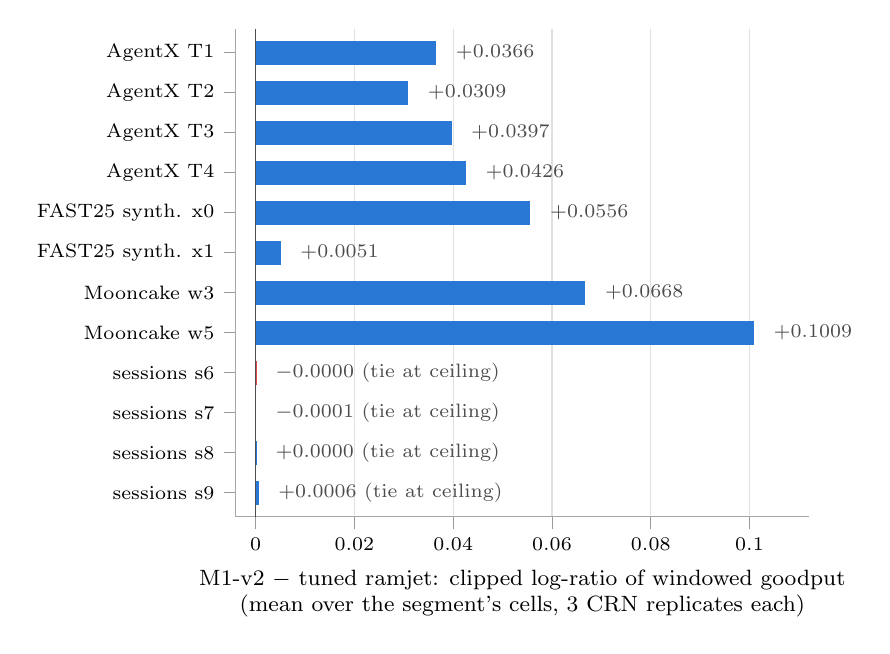
\begin{tikzpicture}
\begin{axis}[
  width=0.6\linewidth, height=6.2cm,
  scale only axis,
  tick label style={font=\scriptsize}, label style={font=\footnotesize, align=center},
  scaled ticks=false, tick label style={/pgf/number format/fixed},
  tick align=outside, tick style={black!40}, axis line style={black!35},
  axis x line*=bottom, axis y line*=left,
  grid style={black!12, line width=0.4pt},
  legend style={font=\scriptsize, draw=none, fill=white, fill opacity=0.85, text opacity=1},
  legend cell align=left,
  y dir=reverse, ymin=-0.6, ymax=11.6,
  ytick={0,1,2,3,4,5,6,7,8,9,10,11},
  yticklabels={{AgentX T1},{AgentX T2},{AgentX T3},{AgentX T4},{FAST25 synth. x0},{FAST25 synth. x1},{Mooncake w3},{Mooncake w5},{sessions s6},{sessions s7},{sessions s8},{sessions s9}},
  xmin=-0.004, xmax=0.112, xtick={0,0.02,0.04,0.06,0.08,0.1}, xmajorgrids,
  xlabel={M1-v2 $-$ tuned \policy{ramjet}: clipped log-ratio of windowed goodput\\(mean over the segment's cells, 3 CRN replicates each)},
  clip=false,
]
% data: segment.agentx:T1
\addplot[xbar, bar shift=0pt, bar width=0.6, fill={rgb,255:red,42;green,120;blue,214}, draw=none, forget plot] coordinates {(0.03657445080582166,0.0)};
\node[anchor=west, font=\scriptsize, text=black!70] at (axis cs:0.03857445080582166,0) {$+$0.0366};
% data: segment.agentx:T2
\addplot[xbar, bar shift=0pt, bar width=0.6, fill={rgb,255:red,42;green,120;blue,214}, draw=none, forget plot] coordinates {(0.030891964057639762,1.0)};
\node[anchor=west, font=\scriptsize, text=black!70] at (axis cs:0.032891964057639764,1) {$+$0.0309};
% data: segment.agentx:T3
\addplot[xbar, bar shift=0pt, bar width=0.6, fill={rgb,255:red,42;green,120;blue,214}, draw=none, forget plot] coordinates {(0.039670656703564705,2.0)};
\node[anchor=west, font=\scriptsize, text=black!70] at (axis cs:0.04167065670356471,2) {$+$0.0397};
% data: segment.agentx:T4
\addplot[xbar, bar shift=0pt, bar width=0.6, fill={rgb,255:red,42;green,120;blue,214}, draw=none, forget plot] coordinates {(0.04260327715057185,3.0)};
\node[anchor=west, font=\scriptsize, text=black!70] at (axis cs:0.04460327715057185,3) {$+$0.0426};
% data: segment.fast25_synthetic:x0
\addplot[xbar, bar shift=0pt, bar width=0.6, fill={rgb,255:red,42;green,120;blue,214}, draw=none, forget plot] coordinates {(0.05564320539796931,4.0)};
\node[anchor=west, font=\scriptsize, text=black!70] at (axis cs:0.05764320539796931,4) {$+$0.0556};
% data: segment.fast25_synthetic:x1
\addplot[xbar, bar shift=0pt, bar width=0.6, fill={rgb,255:red,42;green,120;blue,214}, draw=none, forget plot] coordinates {(0.005070687323773607,5.0)};
\node[anchor=west, font=\scriptsize, text=black!70] at (axis cs:0.007070687323773607,5) {$+$0.0051};
% data: segment.mooncake:w3
\addplot[xbar, bar shift=0pt, bar width=0.6, fill={rgb,255:red,42;green,120;blue,214}, draw=none, forget plot] coordinates {(0.06675942233864367,6.0)};
\node[anchor=west, font=\scriptsize, text=black!70] at (axis cs:0.06875942233864367,6) {$+$0.0668};
% data: segment.mooncake:w5
\addplot[xbar, bar shift=0pt, bar width=0.6, fill={rgb,255:red,42;green,120;blue,214}, draw=none, forget plot] coordinates {(0.10091757894281667,7.0)};
\node[anchor=west, font=\scriptsize, text=black!70] at (axis cs:0.10291757894281667,7) {$+$0.1009};
% data: segment.sessions:s6
\addplot[xbar, bar shift=0pt, bar width=0.6, fill={rgb,255:red,227;green,73;blue,72}, draw=none, forget plot] coordinates {(-1.4614822423291105e-05,8.0)};
\node[anchor=west, font=\scriptsize, text=black!70] at (axis cs:0.002,8) {$-$0.0000 (tie at ceiling)};
% data: segment.sessions:s7
\addplot[xbar, bar shift=0pt, bar width=0.6, fill={rgb,255:red,227;green,73;blue,72}, draw=none, forget plot] coordinates {(-9.739391293188315e-05,9.0)};
\node[anchor=west, font=\scriptsize, text=black!70] at (axis cs:0.002,9) {$-$0.0001 (tie at ceiling)};
% data: segment.sessions:s8
\addplot[xbar, bar shift=0pt, bar width=0.6, fill={rgb,255:red,42;green,120;blue,214}, draw=none, forget plot] coordinates {(4.53237917723111e-05,10.0)};
\node[anchor=west, font=\scriptsize, text=black!70] at (axis cs:0.0020453237917723113,10) {$+$0.0000 (tie at ceiling)};
% data: segment.sessions:s9
\addplot[xbar, bar shift=0pt, bar width=0.6, fill={rgb,255:red,42;green,120;blue,214}, draw=none, forget plot] coordinates {(0.000593503710295625,11.0)};
\node[anchor=west, font=\scriptsize, text=black!70] at (axis cs:0.002593503710295625,11) {$+$0.0006 (tie at ceiling)};
\draw[black!70, line width=0.6pt] ({axis cs:0.0,0} |- {rel axis cs:0,0}) -- ({axis cs:0.0,0} |- {rel axis cs:0,1});
\end{axis}
\end{tikzpicture}

  % src: CR/report/data/report_data.json comparisons.ramjet.m1v2.all.by_segment, drawn by
  %      scripts/make_figures.py (formerly fig/headline_segments.png, report figure F1)
  \caption{The headline per test segment, labeled by family and the segment names of
    \cref{tab:headline}. The four session segments tie at ceiling;
    every other segment favors M1-v2.}
  \label{fig:headline}
\end{figure}

\begin{figure}[tbp]
  \centering
  % GENERATED by scripts/make_figures.py from report/data/report_data.json. Do not edit; regenerate.
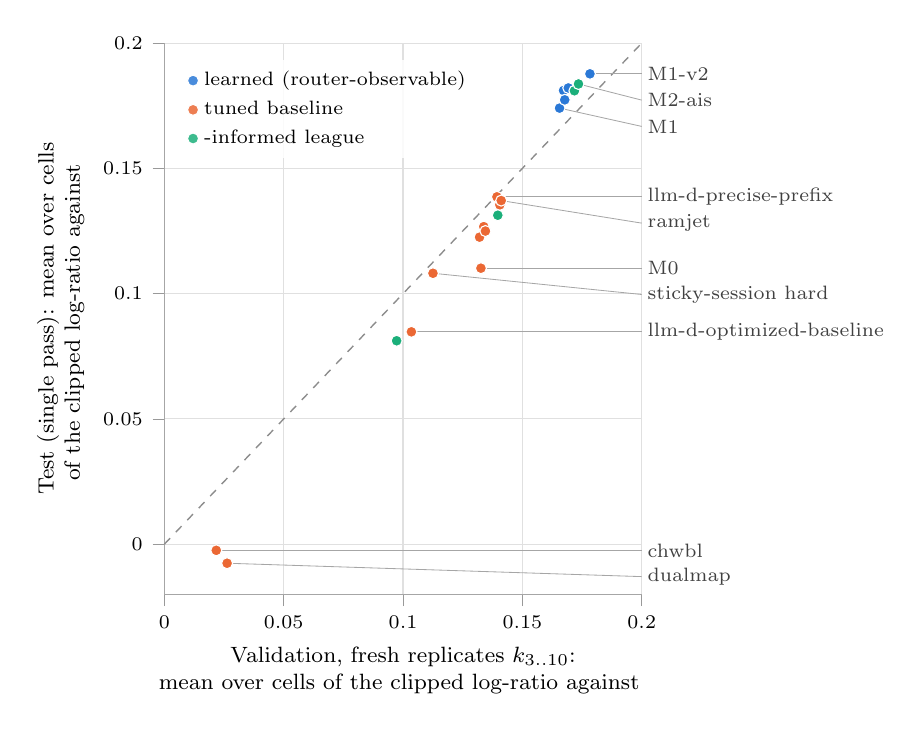
\begin{tikzpicture}
\begin{axis}[
  width=0.5\linewidth, height=7.0cm, xmin=0, xmax=0.2, ymin=-0.02, ymax=0.2,
  scale only axis,
  tick label style={font=\scriptsize}, label style={font=\footnotesize, align=center},
  scaled ticks=false, tick label style={/pgf/number format/fixed},
  tick align=outside, tick style={black!40}, axis line style={black!35},
  axis x line*=bottom, axis y line*=left,
  grid style={black!12, line width=0.4pt},
  legend style={font=\scriptsize, draw=none, fill=white, fill opacity=0.85, text opacity=1},
  legend cell align=left,
  xmajorgrids, ymajorgrids,
  xlabel={Validation, fresh replicates $k_{3..10}$:\\mean over cells of the clipped log-ratio against $\piref$},
  ylabel={Test (single pass): mean over cells\\of the clipped log-ratio against $\piref$},
  legend style={at={(0.03,0.97)}, anchor=north west},
  clip=false,
]
\draw[black!45, line width=0.5pt, dashed] (axis cs:0,0) -- (axis cs:0.2,0.2);
% data: points.learned
\addplot[only marks, mark=*, mark size=2pt, color={rgb,255:red,42;green,120;blue,214}, mark options={draw=white, line width=0.4pt}] coordinates {(0.16836845964916694,0.18187320385634786) (0.16556456087816657,0.17406140813739945) (0.167237480661827,0.18110069617862282) (0.1692366009703472,0.18211393631847803) (0.17830748263632787,0.18774355882517585) (0.16774290438003298,0.17736484274621056)};
\addlegendentry{learned (router-observable)}
% data: points.tuned
\addplot[only marks, mark=*, mark size=2pt, color={rgb,255:red,235;green,104;blue,52}, mark options={draw=white, line width=0.4pt}] coordinates {(0.1405424581894374,0.13545848680044134) (0.02175477178467915,-0.0024413414840022663) (0.026285052719892177,-0.007592867432509777) (0.10349998934991964,0.08476994325492675) (0.13933790761239287,0.13864885481765013) (0.1320527687218506,0.12255959766888537) (0.13262963505096179,0.11016641308341514) (0.1411348331803814,0.13715999535272497) (0.13380951224916446,0.12675376843750322) (0.1125374192869206,0.10814567458942412) (0.13451775465167037,0.12499168901633646)};
\addlegendentry{tuned baseline}
% data: points.ais
\addplot[only marks, mark=*, mark size=2pt, color={rgb,255:red,27;green,175;blue,122}, mark options={draw=white, line width=0.4pt}] coordinates {(0.09732607832444609,0.08120001427607196) (0.13970245464408904,0.13130833932846517) (0.17180490670878812,0.18097536262899377) (0.17350843809790512,0.18370126112559385)};
\addlegendentry{\ais{}-informed league}
\draw[black!35, line width=0.3pt] (axis cs:0.17830748263632787,0.18774355882517585) -- ({rel axis cs:1,0} |- {axis cs:0,0.18774355882517585}) node[anchor=west, xshift=1pt, font=\scriptsize, text=black!75, inner sep=1pt] {M1-v2};
\draw[black!35, line width=0.3pt] (axis cs:0.17350843809790512,0.18370126112559385) -- ({rel axis cs:1,0} |- {axis cs:0,0.17724995264469284}) node[anchor=west, xshift=1pt, font=\scriptsize, text=black!75, inner sep=1pt] {M2-ais};
\draw[black!35, line width=0.3pt] (axis cs:0.16556456087816657,0.17406140813739945) -- ({rel axis cs:1,0} |- {axis cs:0,0.16675634646420984}) node[anchor=west, xshift=1pt, font=\scriptsize, text=black!75, inner sep=1pt] {M1};
\draw[black!35, line width=0.3pt] (axis cs:0.13933790761239287,0.13864885481765013) -- ({rel axis cs:1,0} |- {axis cs:0,0.13864885481765013}) node[anchor=west, xshift=1pt, font=\scriptsize, text=black!75, inner sep=1pt] {llm-d-precise-prefix};
\draw[black!35, line width=0.3pt] (axis cs:0.1411348331803814,0.13715999535272497) -- ({rel axis cs:1,0} |- {axis cs:0,0.12815524863716712}) node[anchor=west, xshift=1pt, font=\scriptsize, text=black!75, inner sep=1pt] {ramjet};
\draw[black!35, line width=0.3pt] (axis cs:0.13262963505096179,0.11016641308341514) -- ({rel axis cs:1,0} |- {axis cs:0,0.11016641308341514}) node[anchor=west, xshift=1pt, font=\scriptsize, text=black!75, inner sep=1pt] {M0};
\draw[black!35, line width=0.3pt] (axis cs:0.1125374192869206,0.10814567458942412) -- ({rel axis cs:1,0} |- {axis cs:0,0.09967280690293215}) node[anchor=west, xshift=1pt, font=\scriptsize, text=black!75, inner sep=1pt] {sticky-session hard};
\draw[black!35, line width=0.3pt] (axis cs:0.10349998934991964,0.08476994325492675) -- ({rel axis cs:1,0} |- {axis cs:0,0.08476994325492675}) node[anchor=west, xshift=1pt, font=\scriptsize, text=black!75, inner sep=1pt] {llm-d-optimized-baseline};
\draw[black!35, line width=0.3pt] (axis cs:0.02175477178467915,-0.0024413414840022663) -- ({rel axis cs:1,0} |- {axis cs:0,-0.0024413414840022663}) node[anchor=west, xshift=1pt, font=\scriptsize, text=black!75, inner sep=1pt] {chwbl};
\draw[black!35, line width=0.3pt] (axis cs:0.026285052719892177,-0.007592867432509777) -- ({rel axis cs:1,0} |- {axis cs:0,-0.012934947664485262}) node[anchor=west, xshift=1pt, font=\scriptsize, text=black!75, inner sep=1pt] {dualmap};
\end{axis}
\end{tikzpicture}

  % src: CR/report/data/report_data.json val_k3_10.<policy> and
  %      comparisons.default.<policy>.all.cell_mean, drawn by scripts/make_figures.py (formerly
  %      fig/val_vs_test.png, report figure F7; the same ten policies are labeled)
  \caption{Validation (fresh replicates) against test, mean over cells of the clipped log-ratio
    against $\piref$. The two compare different cells, so the dashed line is a reference, not an
    expectation.}
  \label{fig:val-test}
\end{figure}

\begin{table}[tbp]
  \centering
  \caption{Rung-to-rung comparisons on test (descriptive).}
  \label{tab:ladder-pairs}
  % GENERATED by scripts/make_tables.py from the report fragment report/data/tables/ladder_pairs.md.
% Do not edit; regenerate.
{\scriptsize
\begin{adjustbox}{max width=\linewidth}
\begin{tabular}{@{}P{0.46\linewidth}lrrr@{}}
\toprule
Comparison ($A - B$) & Segment mean [95\% CI] & Ahead & $p$ ($A > B$) & Cell mean \\
\midrule
M1 $-$ M0 (default cost fn, tuned) & $+$0.0467 [$+$0.0248, $+$0.0700] & 11/12 & 0.0007 & $+$0.0639 \\
M2 rank 2 $-$ M1 & $+$0.0025 [$-$0.0008, $+$0.0070] & 6/12 & 0.2349 & $+$0.0033 \\
M1 continued (secondary) $-$ M1 & $+$0.0071 [$-$0.0024, $+$0.0195] & 6/12 & 0.3386 & $+$0.0070 \\
M2 rank 2 $-$ M1 continued (secondary) & $-$0.0045 [$-$0.0134, $+$0.0029] & 8/12 & 0.5452 & $-$0.0037 \\
M1-v2 (headline learned arm) $-$ M1 & $+$0.0130 [$+$0.0039, $+$0.0244] & 11/12 & 0.0034 & $+$0.0137 \\
M1-noaff $-$ M1 & $+$0.0084 [$-$0.0012, $+$0.0211] & 7/12 & 0.2119 & $+$0.0081 \\
M1 + queue threshold (ablation) $-$ M1 continued (secondary) & $+$0.0015 [$-$0.0002, $+$0.0035] & 8/12 & 0.0549 & $+$0.0008 \\
ramjet + queue threshold (ablation) $-$ ramjet (val-best baseline) & $-$0.0016 [$-$0.0050, $+$0.0010] & 4/12 & 0.8833 & $-$0.0017 \\
M1 $-$ M1 unconstrained (flagged for gaming) & $+$0.0039 [$-$0.0065, $+$0.0144] & 8/12 & 0.1902 & $+$0.0053 \\
M1-ais $-$ M0-ais & $+$0.0275 [$+$0.0104, $+$0.0486] & 10/12 & 0.0017 & $+$0.0497 \\
M2-ais $-$ M1-ais & $+$0.0030 [$+$0.0010, $+$0.0053] & 9/12 & 0.0046 & $+$0.0027 \\
M2-ais $-$ M1-v2 (headline learned arm) & $-$0.0029 [$-$0.0052, $-$0.0006] & 3/12 & 0.9788 & $-$0.0040 \\
M0-ais $-$ M0 (default cost fn, tuned) & $+$0.0262 [$+$0.0101, $+$0.0445] & 10/12 & 0.0017 & $+$0.0211 \\
\bottomrule
\end{tabular}
\end{adjustbox}}

\end{table}

\begin{figure}[tbp]
  \centering
  % GENERATED by scripts/make_figures.py from report/data/report_data.json. Do not edit; regenerate.
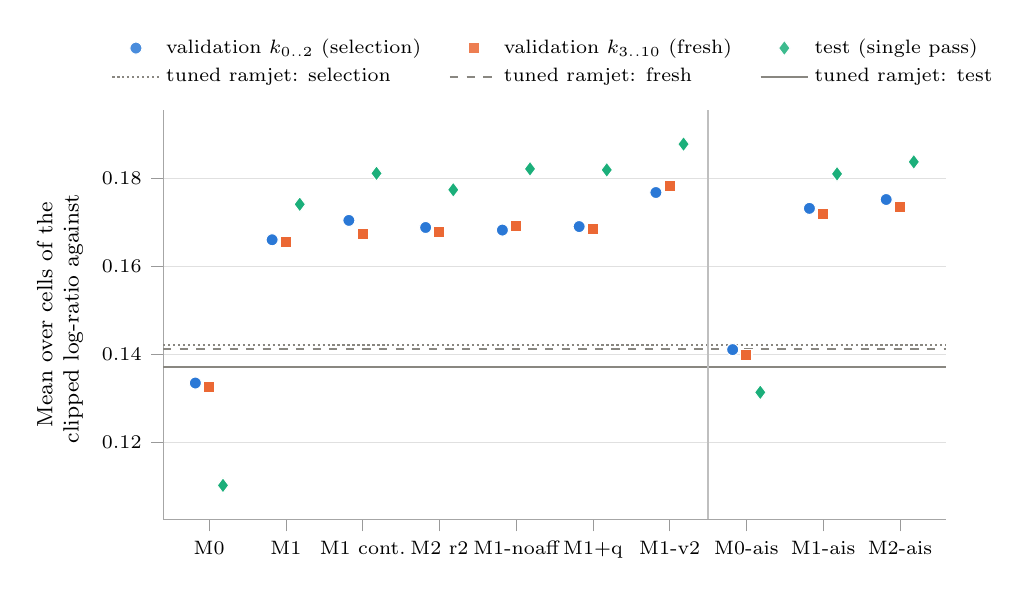
\begin{tikzpicture}
\begin{axis}[
  width=0.82\linewidth, height=5.2cm,
  scale only axis,
  tick label style={font=\scriptsize}, label style={font=\footnotesize, align=center},
  scaled ticks=false, tick label style={/pgf/number format/fixed},
  tick align=outside, tick style={black!40}, axis line style={black!35},
  axis x line*=bottom, axis y line*=left,
  grid style={black!12, line width=0.4pt},
  legend style={font=\scriptsize, draw=none, fill=white, fill opacity=0.85, text opacity=1},
  legend cell align=left,
  xmin=-0.6, xmax=9.6, xtick={0,1,2,3,4,5,6,7,8,9}, xticklabels={{M0},{M1},{M1 cont.},{M2 r2},{M1-noaff},{M1+q},{M1-v2},{M0-ais},{M1-ais},{M2-ais}},
  ymajorgrids, ylabel={Mean over cells of the\\clipped log-ratio against $\piref$},
  legend style={at={(0.5,1.03)}, anchor=south, legend columns=3, /tikz/every even column/.append style={column sep=8pt}},
]
% data: rungs.selection
\addplot[only marks, mark=*, mark size=2.2pt, color={rgb,255:red,42;green,120;blue,214}, mark options={draw=white, line width=0.4pt}] coordinates {(-0.18,0.13342890354099643) (0.8200000000000001,0.16599470141735354) (1.82,0.1704010804209599) (2.82,0.16878966053653194) (3.82,0.16820085589858194) (4.82,0.1690002698298348) (5.82,0.1767435156036474) (6.82,0.14102164778955317) (7.82,0.17313714730249014) (8.82,0.1751499238515255)};
\addlegendentry{validation $k_{0..2}$ (selection)}
% data: rungs.fresh
\addplot[only marks, mark=square*, mark size=2pt, color={rgb,255:red,235;green,104;blue,52}, mark options={draw=white, line width=0.4pt}] coordinates {(0.0,0.13262963505096179) (1.0,0.16556456087816657) (2.0,0.167237480661827) (3.0,0.16774290438003298) (4.0,0.1692366009703472) (5.0,0.16836845964916694) (6.0,0.17830748263632787) (7.0,0.13970245464408904) (8.0,0.17180490670878812) (9.0,0.17350843809790512)};
\addlegendentry{validation $k_{3..10}$ (fresh)}
% data: rungs.test
\addplot[only marks, mark=diamond*, mark size=2.8pt, color={rgb,255:red,27;green,175;blue,122}, mark options={draw=white, line width=0.4pt}] coordinates {(0.18,0.11016641308341514) (1.18,0.17406140813739945) (2.18,0.18110069617862282) (3.18,0.17736484274621056) (4.18,0.18211393631847803) (5.18,0.18187320385634786) (6.18,0.18774355882517585) (7.18,0.13130833932846517) (8.18,0.18097536262899377) (9.18,0.18370126112559385)};
\addlegendentry{test (single pass)}
% data: ramjet.selection
\addplot[color={rgb,255:red,137;green,135;blue,129}, densely dotted, line width=0.8pt, no marks] coordinates {(-0.6,0.14201773497049403) (9.6,0.14201773497049403)};
\addlegendentry{tuned \policy{ramjet}: selection}
% data: ramjet.fresh
\addplot[color={rgb,255:red,137;green,135;blue,129}, dashed, line width=0.8pt, no marks] coordinates {(-0.6,0.1411348331803814) (9.6,0.1411348331803814)};
\addlegendentry{tuned \policy{ramjet}: fresh}
% data: ramjet.test
\addplot[color={rgb,255:red,137;green,135;blue,129}, solid, line width=0.8pt, no marks] coordinates {(-0.6,0.13715999535272497) (9.6,0.13715999535272497)};
\addlegendentry{tuned \policy{ramjet}: test}
\draw[black!25, line width=0.8pt] ({axis cs:6.5,0} |- {rel axis cs:0,0}) -- ({axis cs:6.5,0} |- {rel axis cs:0,1});
\end{axis}
\end{tikzpicture}

  % src: CR/report/data/report_data.json val_k0_2.<arm>, val_k3_10.<arm> and
  %      comparisons.default.<arm>.all.cell_mean (arms and tuned ramjet), drawn by
  %      scripts/make_figures.py (formerly fig/ladder.png, report figure F4)
  \caption{The model ladder on the selection replicates, the fresh validation replicates and test.
    Left of the vertical rule: router-observable arms; right of it: the \ais{}-informed league. ``M1
    cont.'' is M1 continued, ``M2 r2'' is M2 at rank 2 and ``M1+q'' is M1 with the queue threshold.}
  \label{fig:ladder}
\end{figure}

\begin{figure}[tbp]
  \centering
  % GENERATED by scripts/make_figures.py from report/data/report_data.json. Do not edit; regenerate.
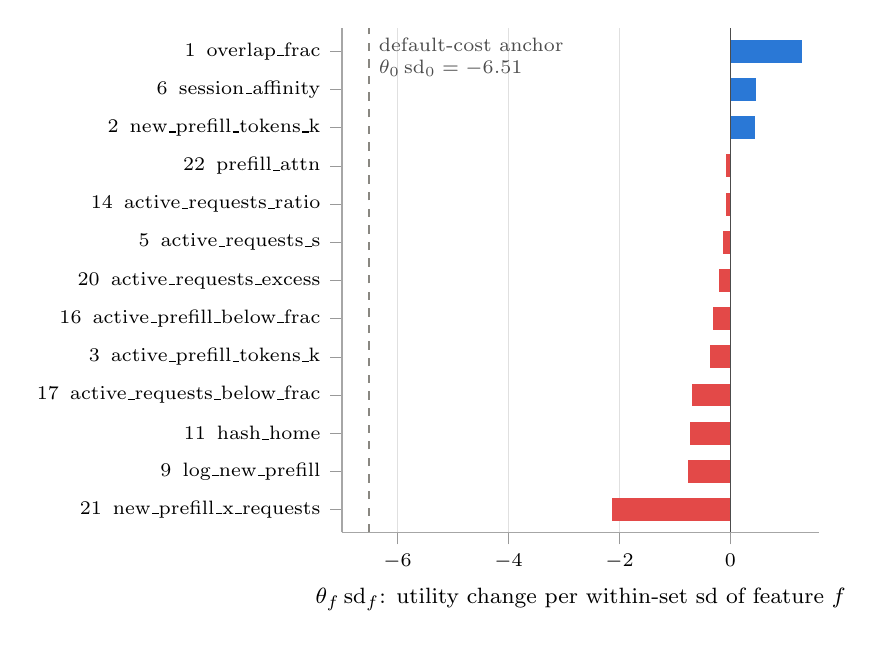
\begin{tikzpicture}
\begin{axis}[
  width=0.5\linewidth, height=6.4cm,
  scale only axis,
  tick label style={font=\scriptsize}, label style={font=\footnotesize, align=center},
  scaled ticks=false, tick label style={/pgf/number format/fixed},
  tick align=outside, tick style={black!40}, axis line style={black!35},
  axis x line*=bottom, axis y line*=left,
  grid style={black!12, line width=0.4pt},
  legend style={font=\scriptsize, draw=none, fill=white, fill opacity=0.85, text opacity=1},
  legend cell align=left,
  ymin=-0.6, ymax=12.6, ytick={0,1,2,3,4,5,6,7,8,9,10,11,12},
  yticklabels={{21\enspace\code{new\_prefill\_x\_requests}},{9\enspace\code{log\_new\_prefill}},{11\enspace\code{hash\_home}},{17\enspace\code{active\_requests\_below\_frac}},{3\enspace\code{active\_prefill\_tokens\_k}},{16\enspace\code{active\_prefill\_below\_frac}},{20\enspace\code{active\_requests\_excess}},{5\enspace\code{active\_requests\_s}},{14\enspace\code{active\_requests\_ratio}},{22\enspace\code{prefill\_attn}},{2\enspace\code{new\_prefill\_tokens\_k}},{6\enspace\code{session\_affinity}},{1\enspace\code{overlap\_frac}}},
  xmin=-7, xmax=1.6, xmajorgrids,
  xlabel={$\theta_f\,\mathrm{sd}_f$: utility change per within-set sd of feature $f$},
  clip=false,
]
% data: coef.21
\addplot[xbar, bar shift=0pt, bar width=0.6, fill={rgb,255:red,227;green,73;blue,72}, draw=none, forget plot] coordinates {(-2.128489075926415,0.0)};
% data: coef.9
\addplot[xbar, bar shift=0pt, bar width=0.6, fill={rgb,255:red,227;green,73;blue,72}, draw=none, forget plot] coordinates {(-0.7623893316636174,1.0)};
% data: coef.11
\addplot[xbar, bar shift=0pt, bar width=0.6, fill={rgb,255:red,227;green,73;blue,72}, draw=none, forget plot] coordinates {(-0.7383408125966545,2.0)};
% data: coef.17
\addplot[xbar, bar shift=0pt, bar width=0.6, fill={rgb,255:red,227;green,73;blue,72}, draw=none, forget plot] coordinates {(-0.6986997281194663,3.0)};
% data: coef.3
\addplot[xbar, bar shift=0pt, bar width=0.6, fill={rgb,255:red,227;green,73;blue,72}, draw=none, forget plot] coordinates {(-0.36126360489603904,4.0)};
% data: coef.16
\addplot[xbar, bar shift=0pt, bar width=0.6, fill={rgb,255:red,227;green,73;blue,72}, draw=none, forget plot] coordinates {(-0.31793560403582644,5.0)};
% data: coef.20
\addplot[xbar, bar shift=0pt, bar width=0.6, fill={rgb,255:red,227;green,73;blue,72}, draw=none, forget plot] coordinates {(-0.20242523761742345,6.0)};
% data: coef.5
\addplot[xbar, bar shift=0pt, bar width=0.6, fill={rgb,255:red,227;green,73;blue,72}, draw=none, forget plot] coordinates {(-0.1287358962783343,7.0)};
% data: coef.14
\addplot[xbar, bar shift=0pt, bar width=0.6, fill={rgb,255:red,227;green,73;blue,72}, draw=none, forget plot] coordinates {(-0.08966912381406741,8.0)};
% data: coef.22
\addplot[xbar, bar shift=0pt, bar width=0.6, fill={rgb,255:red,227;green,73;blue,72}, draw=none, forget plot] coordinates {(-0.08446106952593102,9.0)};
% data: coef.2
\addplot[xbar, bar shift=0pt, bar width=0.6, fill={rgb,255:red,42;green,120;blue,214}, draw=none, forget plot] coordinates {(0.44851952512983045,10.0)};
% data: coef.6
\addplot[xbar, bar shift=0pt, bar width=0.6, fill={rgb,255:red,42;green,120;blue,214}, draw=none, forget plot] coordinates {(0.4513385789422368,11.0)};
% data: coef.1
\addplot[xbar, bar shift=0pt, bar width=0.6, fill={rgb,255:red,42;green,120;blue,214}, draw=none, forget plot] coordinates {(1.289157937216578,12.0)};
% data: anchor
\addplot[color={rgb,255:red,137;green,135;blue,129}, dashed, line width=0.6pt, no marks, forget plot] coordinates {(-6.5099599822061185,-0.6) (-6.5099599822061185,12.6)};
\node[anchor=north west, font=\scriptsize, text=black!70, align=left] at (axis cs:-6.5099599822061185,12.6) {default-cost anchor\\$\theta_0\,\mathrm{sd}_0 = -6.51$};
\draw[black!70, line width=0.6pt] ({axis cs:0.0,0} |- {rel axis cs:0,0}) -- ({axis cs:0.0,0} |- {rel axis cs:0,1});
\end{axis}
\end{tikzpicture}

  % src: CR/report/data/report_data.json coefficients_m1v2 (index, feature,
  %      theta_x_sd), drawn by scripts/make_figures.py (formerly fig/coefficients_m1v2.png, report F6)
  \caption{M1-v2's nonzero coefficients, standardized, labeled with the feature index $f$ and name
    of \cref{tab:coef-m1v2}. Positive attracts a worker, negative repels it; the default-cost
    anchor is at $-6.51$.}
  \label{fig:coef}
\end{figure}

\begin{figure}[tbp]
  \centering
  % GENERATED by scripts/make_figures.py from report/data/report_data.json. Do not edit; regenerate.
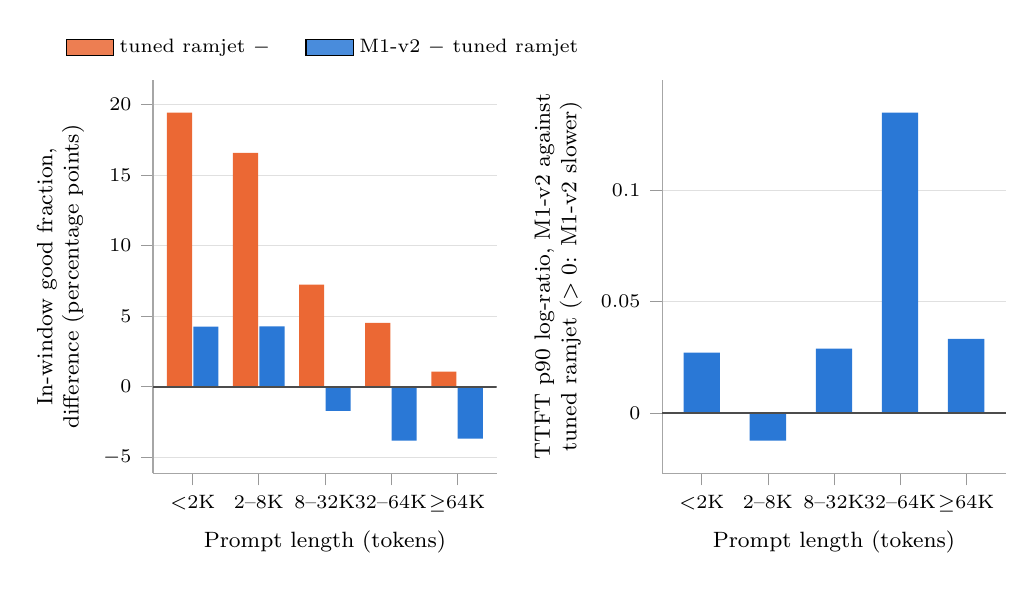
\begin{tikzpicture}
\begin{axis}[
  name=islleft,
  width=0.36\linewidth, height=5cm,
  scale only axis,
  tick label style={font=\scriptsize}, label style={font=\footnotesize, align=center},
  scaled ticks=false, tick label style={/pgf/number format/fixed},
  tick align=outside, tick style={black!40}, axis line style={black!35},
  axis x line*=bottom, axis y line*=left,
  grid style={black!12, line width=0.4pt},
  legend style={font=\scriptsize, draw=none, fill=white, fill opacity=0.85, text opacity=1},
  legend cell align=left,
  xmin=-0.6, xmax=4.6, xtick={0,1,2,3,4}, xticklabels={{$<$2K},{2--8K},{8--32K},{32--64K},{$\geq$64K}},
  xlabel={Prompt length (tokens)}, ymajorgrids,
  yticklabel={\pgfmathparse{100*\tick}\pgfmathprintnumber[fixed, precision=0]{\pgfmathresult}},
  ylabel={In-window good fraction,\\difference (percentage points)},
  legend style={at={(0.5,1.03)}, anchor=south, legend columns=2, /tikz/every even column/.append style={column sep=8pt}},
]
% data: good.ramjet_default
\addplot[ybar, bar shift=0pt, bar width=0.38, fill={rgb,255:red,235;green,104;blue,52}, draw=none, area legend] coordinates {(-0.2,0.194361) (0.8,0.165715) (1.8,0.0724444) (2.8,0.0452659) (3.8,0.0106691)};
\addlegendentry{tuned \policy{ramjet} $-$ $\piref$}
% data: good.m1v2_ramjet
\addplot[ybar, bar shift=0pt, bar width=0.38, fill={rgb,255:red,42;green,120;blue,214}, draw=none, area legend] coordinates {(0.2,0.0425579) (1.2,0.0428022) (2.2,-0.0171906) (3.2,-0.038277) (4.2,-0.0369138)};
\addlegendentry{M1-v2 $-$ tuned \policy{ramjet}}
\draw[black!70, line width=0.6pt] ({rel axis cs:0,0} |- {axis cs:0,0.0}) -- ({rel axis cs:1,0} |- {axis cs:0,0.0});
\end{axis}
\begin{axis}[
  at={(islleft.south east)}, anchor=south west, xshift=2.1cm,
  width=0.36\linewidth, height=5cm,
  scale only axis,
  tick label style={font=\scriptsize}, label style={font=\footnotesize, align=center},
  scaled ticks=false, tick label style={/pgf/number format/fixed},
  tick align=outside, tick style={black!40}, axis line style={black!35},
  axis x line*=bottom, axis y line*=left,
  grid style={black!12, line width=0.4pt},
  legend style={font=\scriptsize, draw=none, fill=white, fill opacity=0.85, text opacity=1},
  legend cell align=left,
  xmin=-0.6, xmax=4.6, xtick={0,1,2,3,4}, xticklabels={{$<$2K},{2--8K},{8--32K},{32--64K},{$\geq$64K}},
  xlabel={Prompt length (tokens)}, ymajorgrids,
  ylabel={TTFT p90 log-ratio, M1-v2 against\\tuned \policy{ramjet} ($>0$: M1-v2 slower)},
]
% data: ttft.m1v2_ramjet
\addplot[ybar, bar shift=0pt, bar width=0.55, fill={rgb,255:red,42;green,120;blue,214}, draw=none, forget plot] coordinates {(0.0,0.0270878) (1.0,-0.0124485) (2.0,0.0288946) (3.0,0.134982) (4.0,0.0332504)};
\draw[black!70, line width=0.6pt] ({rel axis cs:0,0} |- {axis cs:0,0.0}) -- ({rel axis cs:1,0} |- {axis cs:0,0.0});
\end{axis}
\end{tikzpicture}

  % src: CR/report/data/report_data.json isl_buckets.<bucket> (good_ramjet_default,
  %      good_m1v2_ramjet, ttft_m1v2_ramjet: segment_mean), drawn by scripts/make_figures.py
  %      (formerly fig/isl_buckets.png, report figure F10)
  \caption{Where M1-v2's gain comes from (segment means on test). Left: in-window good fraction by
    prompt length in percentage points, \policy{ramjet} minus $\piref$ (orange) and M1-v2 minus
    \policy{ramjet} (blue).
    Right: TTFT p90 log-ratio of M1-v2 against \policy{ramjet}.}
  \label{fig:isl}
\end{figure}

% =====================================================================================
\subsection{Cache pressure}

% src: CR/report/REPORT.md section 4 (Spearman 0.79, 0.71; 1.0-2.7); CR/facts/calibration.json
%      cache_pressure_open_loop lessons ("no split has cells below 0.5")
On the 22 open-loop Mooncake and FAST25 test cells, M1-v2's gain rises with cache pressure: Spearman
$\rho$ 0.79 against $\piref$ and 0.71 against \policy{ramjet} (\cref{fig:cache-pressure}). Pressure
ranges from 1.0 to 2.7, so no test cell has little cache pressure, a design gap calibration recorded
(\cref{sec:calibration}).

\begin{figure}[tbp]
  \centering
  % GENERATED by scripts/make_figures.py from report/data/report_data.json. Do not edit; regenerate.
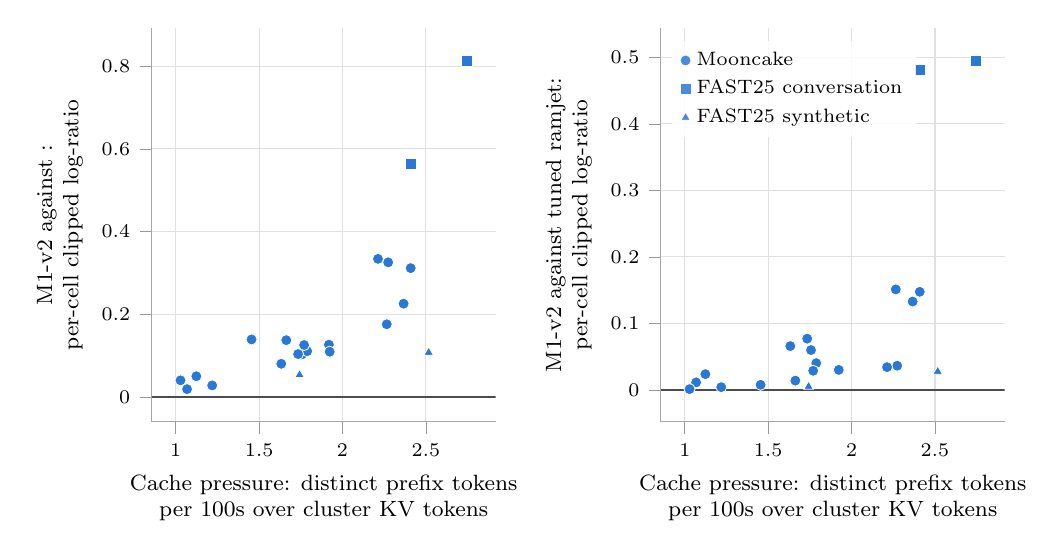
\begin{tikzpicture}
\begin{axis}[
  name=cpleft, width=0.36\linewidth, height=5cm,
  scale only axis,
  tick label style={font=\scriptsize}, label style={font=\footnotesize, align=center},
  scaled ticks=false, tick label style={/pgf/number format/fixed},
  tick align=outside, tick style={black!40}, axis line style={black!35},
  axis x line*=bottom, axis y line*=left,
  grid style={black!12, line width=0.4pt},
  legend style={font=\scriptsize, draw=none, fill=white, fill opacity=0.85, text opacity=1},
  legend cell align=left,
  xmajorgrids, ymajorgrids,
  xlabel={Cache pressure: distinct prefix tokens\\per \SI{100}{s} over cluster KV tokens},
  ylabel={M1-v2 against $\piref$:\\per-cell clipped log-ratio},
  legend style={at={(0.03,0.97)}, anchor=north west},
]
% data: m1v2_vs_default.mooncake
\addplot[only marks, mark=*, mark size=2pt, color={rgb,255:red,42;green,120;blue,214}, mark options={draw=white, line width=0.3pt}] coordinates {(1.662958140449599,0.13708390767366896) (1.0680760685676352,0.018646406968525556) (1.6327814944122352,0.07995279545473953) (1.0286424788258663,0.03989846465962922) (1.4547737975445036,0.13884600978444242) (1.7568570238818544,0.10262799355010817) (1.788177257758446,0.11033075922171198) (1.2187942040011592,0.027547199298678087) (1.7698128964987982,0.12529955098768272) (1.1236368797472236,0.049837815536242724) (2.27379730163919,0.32532798548627595) (2.265171425760735,0.1755062294570351) (2.2126246816380544,0.3336922585193361) (2.3662919853556668,0.22531435015965282) (2.408794738186328,0.31130885052082835) (1.9184876936042667,0.12626656708396325) (1.7338384858513693,0.10350587082541106) (1.9232627723458995,0.1091367587244521)};
% data: m1v2_vs_default.fast25_conversation
\addplot[only marks, mark=square*, mark size=2pt, color={rgb,255:red,42;green,120;blue,214}, mark options={draw=white, line width=0.3pt}] coordinates {(2.410181047818837,0.5636409873887084) (2.7458641097979104,0.8122643249485385)};
% data: m1v2_vs_default.fast25_synthetic
\addplot[only marks, mark=triangle*, mark size=2pt, color={rgb,255:red,42;green,120;blue,214}, mark options={draw=white, line width=0.3pt}] coordinates {(2.5165505977424956,0.10728519098403601) (1.7425118339794181,0.05327629154274147)};
\draw[black!70, line width=0.6pt] ({rel axis cs:0,0} |- {axis cs:0,0.0}) -- ({rel axis cs:1,0} |- {axis cs:0,0.0});
\end{axis}
\begin{axis}[
  at={(cpleft.south east)}, anchor=south west, xshift=2.1cm, width=0.36\linewidth, height=5cm,
  scale only axis,
  tick label style={font=\scriptsize}, label style={font=\footnotesize, align=center},
  scaled ticks=false, tick label style={/pgf/number format/fixed},
  tick align=outside, tick style={black!40}, axis line style={black!35},
  axis x line*=bottom, axis y line*=left,
  grid style={black!12, line width=0.4pt},
  legend style={font=\scriptsize, draw=none, fill=white, fill opacity=0.85, text opacity=1},
  legend cell align=left,
  xmajorgrids, ymajorgrids,
  xlabel={Cache pressure: distinct prefix tokens\\per \SI{100}{s} over cluster KV tokens},
  ylabel={M1-v2 against tuned \policy{ramjet}:\\per-cell clipped log-ratio},
  legend style={at={(0.03,0.97)}, anchor=north west},
]
% data: m1v2_vs_ramjet.mooncake
\addplot[only marks, mark=*, mark size=2pt, color={rgb,255:red,42;green,120;blue,214}, mark options={draw=white, line width=0.3pt}] coordinates {(1.662958140449599,0.014026222433940293) (1.0680760685676352,0.01128173558192431) (1.6327814944122352,0.06588797115852886) (1.0286424788258663,0.001203984777751311) (1.4547737975445036,0.007637622884751107) (1.7568570238818544,0.05990092738100362) (1.788177257758446,0.0402384326279203) (1.2187942040011592,0.004156519149548524) (1.7698128964987982,0.028756639487820635) (1.1236368797472236,0.02371316423989103) (2.27379730163919,0.036397844915040854) (2.265171425760735,0.15108987884710914) (2.2126246816380544,0.03425018661221003) (2.3662919853556668,0.13285757078023258) (2.408794738186328,0.147493683985517) (1.9184876936042667,0.030136199397582886) (1.7338384858513693,0.07705811989834781) (1.9232627723458995,0.030121008600834387)};
\addlegendentry{Mooncake}
% data: m1v2_vs_ramjet.fast25_conversation
\addplot[only marks, mark=square*, mark size=2pt, color={rgb,255:red,42;green,120;blue,214}, mark options={draw=white, line width=0.3pt}] coordinates {(2.410181047818837,0.481465018099776) (2.7458641097979104,0.4943816448038311)};
\addlegendentry{FAST25 conversation}
% data: m1v2_vs_ramjet.fast25_synthetic
\addplot[only marks, mark=triangle*, mark size=2pt, color={rgb,255:red,42;green,120;blue,214}, mark options={draw=white, line width=0.3pt}] coordinates {(2.5165505977424956,0.027708508068614426) (1.7425118339794181,0.005070687323773607)};
\addlegendentry{FAST25 synthetic}
\draw[black!70, line width=0.6pt] ({rel axis cs:0,0} |- {axis cs:0,0.0}) -- ({rel axis cs:1,0} |- {axis cs:0,0.0});
\end{axis}
\end{tikzpicture}

  % src: CR/report/data/report_data.json cache_pressure.cells (pressure,
  %      m1v2_vs_default, m1v2_vs_ramjet, family), drawn by scripts/make_figures.py (formerly
  %      fig/cache_pressure.png, report figure F9)
  \caption{Per-cell gain against cache pressure on the 22 open-loop Mooncake and FAST25 test cells.
    Cache pressure is distinct prefix tokens per \SI{100}{s} over
    the cluster's KV capacity. The trend is descriptive: pressure is confounded with load level, and
    cells of one segment are not independent. Left: against $\piref$; right: against tuned
    \policy{ramjet}; marker shape: family.}
  \label{fig:cache-pressure}
\end{figure}

% =====================================================================================
\subsection{Robustness details}

\Cref{fig:robustness} plots \cref{tab:robustness}.

\begin{figure}[tbp]
  \centering
  % GENERATED by scripts/make_figures.py from report/data/report_data.json. Do not edit; regenerate.
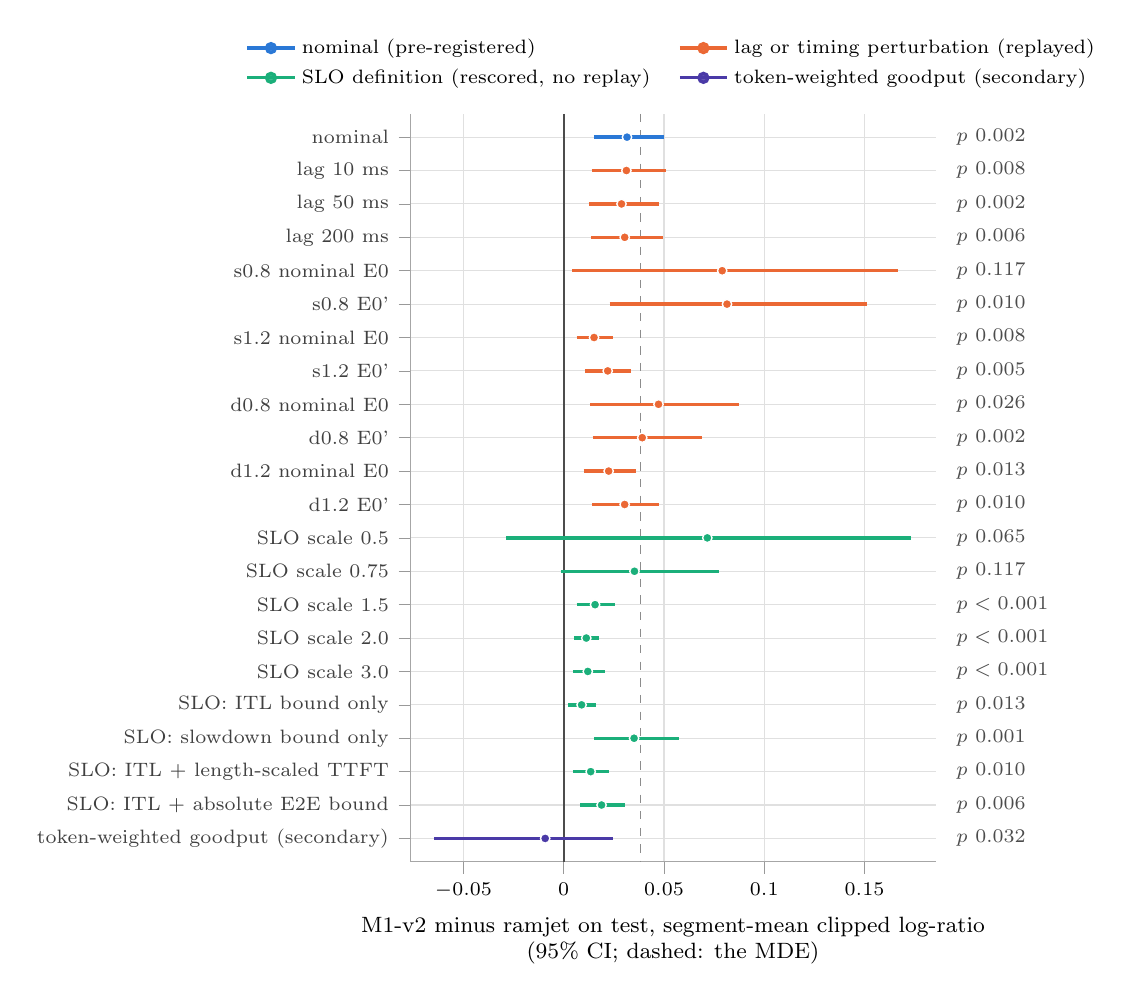
\begin{tikzpicture}
\begin{axis}[
  scale only axis, width=0.55\linewidth, height=9.5cm,
  y dir=reverse, ymin=-0.7, ymax=21.7,
  ytick={0,1,2,3,4,5,6,7,8,9,10,11,12,13,14,15,16,17,18,19,20,21}, yticklabels={{nominal},{lag 10 ms},{lag 50 ms},{lag 200 ms},{s0.8 nominal E0},{s0.8 E0'},{s1.2 nominal E0},{s1.2 E0'},{d0.8 nominal E0},{d0.8 E0'},{d1.2 nominal E0},{d1.2 E0'},{SLO scale 0.5},{SLO scale 0.75},{SLO scale 1.5},{SLO scale 2.0},{SLO scale 3.0},{SLO: ITL bound only},{SLO: slowdown bound only},{SLO: ITL + length-scaled TTFT},{SLO: ITL + absolute E2E bound},{token-weighted goodput (secondary)}},
  yticklabel style={font=\scriptsize, text=black!75}, xticklabel style={font=\scriptsize},
  scaled x ticks=false, xticklabel style={/pgf/number format/fixed},
  tick align=outside, tick style={black!40}, axis line style={black!35},
  axis x line*=bottom, axis y line*=left,
  xmajorgrids, ymajorgrids, grid style={black!12, line width=0.4pt},
  enlarge x limits={abs=0.012},
  xlabel={M1-v2 minus ramjet on test, segment-mean clipped log-ratio\\(95\% CI; dashed: the MDE)}, xlabel style={font=\footnotesize, align=center},
  legend style={font=\scriptsize, draw=none, fill=white, fill opacity=0.85, text opacity=1, at={(0.5,1.02)}, anchor=south, legend columns=2, /tikz/every even column/.append style={column sep=8pt}},
  legend cell align=left,
  clip=false,
]
\addlegendimage{color={rgb,255:red,42;green,120;blue,214}, line width=1.2pt, mark=*, mark size=1.6pt}
\addlegendentry{nominal (pre-registered)}
\addlegendimage{color={rgb,255:red,235;green,104;blue,52}, line width=1.2pt, mark=*, mark size=1.6pt}
\addlegendentry{lag or timing perturbation (replayed)}
\addlegendimage{color={rgb,255:red,27;green,175;blue,122}, line width=1.2pt, mark=*, mark size=1.6pt}
\addlegendentry{SLO definition (rescored, no replay)}
\addlegendimage{color={rgb,255:red,74;green,58;blue,167}, line width=1.2pt, mark=*, mark size=1.6pt}
\addlegendentry{token-weighted goodput (secondary)}
\draw[black!70, line width=0.6pt] (axis cs:0,-0.7) -- (axis cs:0,21.7);
\draw[black!45, line width=0.5pt, dashed] (axis cs:0.03815,-0.7) -- (axis cs:0.03815,21.7);
% row 0: nominal
\addplot[color={rgb,255:red,42;green,120;blue,214}, line width=1.2pt, forget plot] coordinates {(0.015048329896061034,0) (0.05007133566721252,0)};
\addplot[color={rgb,255:red,42;green,120;blue,214}, only marks, mark=*, mark size=1.7pt, mark options={draw=white, line width=0.5pt}, forget plot] coordinates {(0.03155483845729284,0)};
\node[anchor=west, font=\scriptsize, text=black!70, xshift=4pt] at ({rel axis cs:1,0} |- {axis cs:0,0}) {$p$ 0.002};
% row 1: lag 10 ms
\addplot[color={rgb,255:red,235;green,104;blue,52}, line width=1.2pt, forget plot] coordinates {(0.013873275540505924,1) (0.050805064082745086,1)};
\addplot[color={rgb,255:red,235;green,104;blue,52}, only marks, mark=*, mark size=1.7pt, mark options={draw=white, line width=0.5pt}, forget plot] coordinates {(0.031244621199186622,1)};
\node[anchor=west, font=\scriptsize, text=black!70, xshift=4pt] at ({rel axis cs:1,0} |- {axis cs:0,1}) {$p$ 0.008};
% row 2: lag 50 ms
\addplot[color={rgb,255:red,235;green,104;blue,52}, line width=1.2pt, forget plot] coordinates {(0.012499170125988376,2) (0.047736183936878646,2)};
\addplot[color={rgb,255:red,235;green,104;blue,52}, only marks, mark=*, mark size=1.7pt, mark options={draw=white, line width=0.5pt}, forget plot] coordinates {(0.028810805911032297,2)};
\node[anchor=west, font=\scriptsize, text=black!70, xshift=4pt] at ({rel axis cs:1,0} |- {axis cs:0,2}) {$p$ 0.002};
% row 3: lag 200 ms
\addplot[color={rgb,255:red,235;green,104;blue,52}, line width=1.2pt, forget plot] coordinates {(0.013494838317434919,3) (0.04967992554589424,3)};
\addplot[color={rgb,255:red,235;green,104;blue,52}, only marks, mark=*, mark size=1.7pt, mark options={draw=white, line width=0.5pt}, forget plot] coordinates {(0.030401144485522932,3)};
\node[anchor=west, font=\scriptsize, text=black!70, xshift=4pt] at ({rel axis cs:1,0} |- {axis cs:0,3}) {$p$ 0.006};
% row 4: s0.8 nominal E0
\addplot[color={rgb,255:red,235;green,104;blue,52}, line width=1.2pt, forget plot] coordinates {(0.004197486914492673,4) (0.16663719363430637,4)};
\addplot[color={rgb,255:red,235;green,104;blue,52}, only marks, mark=*, mark size=1.7pt, mark options={draw=white, line width=0.5pt}, forget plot] coordinates {(0.07901969522162629,4)};
\node[anchor=west, font=\scriptsize, text=black!70, xshift=4pt] at ({rel axis cs:1,0} |- {axis cs:0,4}) {$p$ 0.117};
% row 5: s0.8 E0'
\addplot[color={rgb,255:red,235;green,104;blue,52}, line width=1.2pt, forget plot] coordinates {(0.022856585445627003,5) (0.15113260751374982,5)};
\addplot[color={rgb,255:red,235;green,104;blue,52}, only marks, mark=*, mark size=1.7pt, mark options={draw=white, line width=0.5pt}, forget plot] coordinates {(0.08141737833183699,5)};
\node[anchor=west, font=\scriptsize, text=black!70, xshift=4pt] at ({rel axis cs:1,0} |- {axis cs:0,5}) {$p$ 0.010};
% row 6: s1.2 nominal E0
\addplot[color={rgb,255:red,235;green,104;blue,52}, line width=1.2pt, forget plot] coordinates {(0.006448834453700277,6) (0.024684969119154486,6)};
\addplot[color={rgb,255:red,235;green,104;blue,52}, only marks, mark=*, mark size=1.7pt, mark options={draw=white, line width=0.5pt}, forget plot] coordinates {(0.015114042856582889,6)};
\node[anchor=west, font=\scriptsize, text=black!70, xshift=4pt] at ({rel axis cs:1,0} |- {axis cs:0,6}) {$p$ 0.008};
% row 7: s1.2 E0'
\addplot[color={rgb,255:red,235;green,104;blue,52}, line width=1.2pt, forget plot] coordinates {(0.010518368143539021,7) (0.03330975694275913,7)};
\addplot[color={rgb,255:red,235;green,104;blue,52}, only marks, mark=*, mark size=1.7pt, mark options={draw=white, line width=0.5pt}, forget plot] coordinates {(0.021922518648143863,7)};
\node[anchor=west, font=\scriptsize, text=black!70, xshift=4pt] at ({rel axis cs:1,0} |- {axis cs:0,7}) {$p$ 0.005};
% row 8: d0.8 nominal E0
\addplot[color={rgb,255:red,235;green,104;blue,52}, line width=1.2pt, forget plot] coordinates {(0.013107551607795604,8) (0.0872491791321521,8)};
\addplot[color={rgb,255:red,235;green,104;blue,52}, only marks, mark=*, mark size=1.7pt, mark options={draw=white, line width=0.5pt}, forget plot] coordinates {(0.04725791730757501,8)};
\node[anchor=west, font=\scriptsize, text=black!70, xshift=4pt] at ({rel axis cs:1,0} |- {axis cs:0,8}) {$p$ 0.026};
% row 9: d0.8 E0'
\addplot[color={rgb,255:red,235;green,104;blue,52}, line width=1.2pt, forget plot] coordinates {(0.014450639385188568,9) (0.0690827883738156,9)};
\addplot[color={rgb,255:red,235;green,104;blue,52}, only marks, mark=*, mark size=1.7pt, mark options={draw=white, line width=0.5pt}, forget plot] coordinates {(0.03914676427295776,9)};
\node[anchor=west, font=\scriptsize, text=black!70, xshift=4pt] at ({rel axis cs:1,0} |- {axis cs:0,9}) {$p$ 0.002};
% row 10: d1.2 nominal E0
\addplot[color={rgb,255:red,235;green,104;blue,52}, line width=1.2pt, forget plot] coordinates {(0.009932519414276307,10) (0.03600649473284267,10)};
\addplot[color={rgb,255:red,235;green,104;blue,52}, only marks, mark=*, mark size=1.7pt, mark options={draw=white, line width=0.5pt}, forget plot] coordinates {(0.022401302732434084,10)};
\node[anchor=west, font=\scriptsize, text=black!70, xshift=4pt] at ({rel axis cs:1,0} |- {axis cs:0,10}) {$p$ 0.013};
% row 11: d1.2 E0'
\addplot[color={rgb,255:red,235;green,104;blue,52}, line width=1.2pt, forget plot] coordinates {(0.014048032085380977,11) (0.047711895977829544,11)};
\addplot[color={rgb,255:red,235;green,104;blue,52}, only marks, mark=*, mark size=1.7pt, mark options={draw=white, line width=0.5pt}, forget plot] coordinates {(0.030378248283595585,11)};
\node[anchor=west, font=\scriptsize, text=black!70, xshift=4pt] at ({rel axis cs:1,0} |- {axis cs:0,11}) {$p$ 0.010};
% row 12: SLO scale 0.5
\addplot[color={rgb,255:red,27;green,175;blue,122}, line width=1.2pt, forget plot] coordinates {(-0.028851322210603117,12) (0.17340884451238658,12)};
\addplot[color={rgb,255:red,27;green,175;blue,122}, only marks, mark=*, mark size=1.7pt, mark options={draw=white, line width=0.5pt}, forget plot] coordinates {(0.07160289781688232,12)};
\node[anchor=west, font=\scriptsize, text=black!70, xshift=4pt] at ({rel axis cs:1,0} |- {axis cs:0,12}) {$p$ 0.065};
% row 13: SLO scale 0.75
\addplot[color={rgb,255:red,27;green,175;blue,122}, line width=1.2pt, forget plot] coordinates {(-0.0014857072287875115,13) (0.07761681795872231,13)};
\addplot[color={rgb,255:red,27;green,175;blue,122}, only marks, mark=*, mark size=1.7pt, mark options={draw=white, line width=0.5pt}, forget plot] coordinates {(0.03527420796349124,13)};
\node[anchor=west, font=\scriptsize, text=black!70, xshift=4pt] at ({rel axis cs:1,0} |- {axis cs:0,13}) {$p$ 0.117};
% row 14: SLO scale 1.5
\addplot[color={rgb,255:red,27;green,175;blue,122}, line width=1.2pt, forget plot] coordinates {(0.006419423835251074,14) (0.025581664260418656,14)};
\addplot[color={rgb,255:red,27;green,175;blue,122}, only marks, mark=*, mark size=1.7pt, mark options={draw=white, line width=0.5pt}, forget plot] coordinates {(0.01562377863823426,14)};
\node[anchor=west, font=\scriptsize, text=black!70, xshift=4pt] at ({rel axis cs:1,0} |- {axis cs:0,14}) {$p < 0.001$};
% row 15: SLO scale 2.0
\addplot[color={rgb,255:red,27;green,175;blue,122}, line width=1.2pt, forget plot] coordinates {(0.005175975444167631,15) (0.017767236573044805,15)};
\addplot[color={rgb,255:red,27;green,175;blue,122}, only marks, mark=*, mark size=1.7pt, mark options={draw=white, line width=0.5pt}, forget plot] coordinates {(0.01125014178980994,15)};
\node[anchor=west, font=\scriptsize, text=black!70, xshift=4pt] at ({rel axis cs:1,0} |- {axis cs:0,15}) {$p < 0.001$};
% row 16: SLO scale 3.0
\addplot[color={rgb,255:red,27;green,175;blue,122}, line width=1.2pt, forget plot] coordinates {(0.004795387304961966,16) (0.02068684403136759,16)};
\addplot[color={rgb,255:red,27;green,175;blue,122}, only marks, mark=*, mark size=1.7pt, mark options={draw=white, line width=0.5pt}, forget plot] coordinates {(0.012003442821919813,16)};
\node[anchor=west, font=\scriptsize, text=black!70, xshift=4pt] at ({rel axis cs:1,0} |- {axis cs:0,16}) {$p < 0.001$};
% row 17: A14 itl_only
\addplot[color={rgb,255:red,27;green,175;blue,122}, line width=1.2pt, forget plot] coordinates {(0.0022376140559881735,17) (0.016066093913023057,17)};
\addplot[color={rgb,255:red,27;green,175;blue,122}, only marks, mark=*, mark size=1.7pt, mark options={draw=white, line width=0.5pt}, forget plot] coordinates {(0.008900876505338292,17)};
\node[anchor=west, font=\scriptsize, text=black!70, xshift=4pt] at ({rel axis cs:1,0} |- {axis cs:0,17}) {$p$ 0.013};
% row 18: A14 e2e_only
\addplot[color={rgb,255:red,27;green,175;blue,122}, line width=1.2pt, forget plot] coordinates {(0.015181117169736906,18) (0.05743971969398245,18)};
\addplot[color={rgb,255:red,27;green,175;blue,122}, only marks, mark=*, mark size=1.7pt, mark options={draw=white, line width=0.5pt}, forget plot] coordinates {(0.03507631457200858,18)};
\node[anchor=west, font=\scriptsize, text=black!70, xshift=4pt] at ({rel axis cs:1,0} |- {axis cs:0,18}) {$p$ 0.001};
% row 19: A14 ttft_len_itl
\addplot[color={rgb,255:red,27;green,175;blue,122}, line width=1.2pt, forget plot] coordinates {(0.004550951496120191,19) (0.02267402128399381,19)};
\addplot[color={rgb,255:red,27;green,175;blue,122}, only marks, mark=*, mark size=1.7pt, mark options={draw=white, line width=0.5pt}, forget plot] coordinates {(0.013442865389640894,19)};
\node[anchor=west, font=\scriptsize, text=black!70, xshift=4pt] at ({rel axis cs:1,0} |- {axis cs:0,19}) {$p$ 0.010};
% row 20: A14 abs_e2e_itl
\addplot[color={rgb,255:red,27;green,175;blue,122}, line width=1.2pt, forget plot] coordinates {(0.008192057395154705,20) (0.030341642406306386,20)};
\addplot[color={rgb,255:red,27;green,175;blue,122}, only marks, mark=*, mark size=1.7pt, mark options={draw=white, line width=0.5pt}, forget plot] coordinates {(0.01886753126534225,20)};
\node[anchor=west, font=\scriptsize, text=black!70, xshift=4pt] at ({rel axis cs:1,0} |- {axis cs:0,20}) {$p$ 0.006};
% row 21: A19 good tokens (secondary)
\addplot[color={rgb,255:red,74;green,58;blue,167}, line width=1.2pt, forget plot] coordinates {(-0.06445106563362452,21) (0.024418716177894567,21)};
\addplot[color={rgb,255:red,74;green,58;blue,167}, only marks, mark=*, mark size=1.7pt, mark options={draw=white, line width=0.5pt}, forget plot] coordinates {(-0.009247690426442193,21)};
\node[anchor=west, font=\scriptsize, text=black!70, xshift=4pt] at ({rel axis cs:1,0} |- {axis cs:0,21}) {$p$ 0.032};
\end{axis}
\end{tikzpicture}

  % src: CR/report/data/report_data.json robustness.<condition> (segment_mean, ci95,
  %      wilcoxon_one_sided_p), drawn by scripts/make_figures.py with the table labels (formerly
  %      fig/robustness.png, report figure F5)
  \caption{The headline under perturbations and alternative SLOs (dashed: the MDE). The four
    ``SLO:'' rows are the alternative SLO definitions, and the last row is the token-weighted
    secondary metric.}
  % prov: the report's labels were "A14 <variant>" and "A19 good tokens (secondary)"
  \label{fig:robustness}
\end{figure}

\paragraph{Lag-0 identity.}
% src: CR/facts/robustness.json lag0_identity_lag_build_vs_tuning_build; CR/audits/final/refute-headline-3.md
%      (lag0 448/448)
The lag build reproduces the tuning build at lag 0 per request: 180 of 180 test records for $\piref$
and M1, and 448 of 448 validation records for M1-v2, \policy{ramjet}, \policy{llm-d-precise-prefix}
and $\piref$ (\cref{sec:robustness}).

\paragraph{Simulator-model counterfactuals.}
% src: CR/audits/final/refute-headline-3.md (simulator model variants); CR/report/REPORT.md section 7.1;
%      CR/facts/UPSTREAM_FOLLOWUPS.md #17
%      (AISim, the replay engine, prices a mixed prefill pass; it calls AIS predict_prefill on batch means)
On validation only, an audit-only \aisim{} build changes how the simulator prices mixed prefill
and decode passes. Against $+0.0290$ on the unmodified simulator, M1-v2's lead over \policy{ramjet} is
$+0.0274$ when mixed prefill passes are priced attention-equivalent, $+0.0291$ when priced as a
per-request sum, $+0.0268$ with an extra \SI{0.1}{ms} of decode cost per running sequence, and
$+0.0269$ when decode inside a prefill pass costs a quarter. These bracket fidelity errors that act
on M1-v2's concentration mechanism; they are not measurements of reality, and FAST25, a test-only
family, is not covered.

% =====================================================================================
\subsection{Herding guards}

% src: generated/tau_hashhome.tex; CR/facts/robustness.json m1_lr14_variants; CR/report/REPORT.md section 7.2
Two guards against herding were registered before M1-v2 won, so they ran as variants of M1
(\cref{app:protocol}; \cref{tab:tau-hashhome}). A positive temperature does not help:
$\temp = 0.747$ is within noise of M1, and $\temp = 2.75$ costs 0.028, more at $\Nw = 16$ and 32
than at 2, as expected when the softmax mass on non-best workers grows with $\Nw$. Restricting
candidates to the prefix's \code{hash\_home} pair is harmful at large $\Nw$ ($-0.57$ at 16 and
$-0.68$ at 32); at $\Nw = 2$ every worker is home, so the variant is identical there. No herding
failure of the argmax appeared under the tested lags in replay.

\begin{table}[tbp]
  \centering
  \caption{Herding guards, as variants of M1 on the lag build at lag 0: segment-mean
    clipped log-ratio against M1 with 95\% intervals, over all test cells and at the unseen worker
    counts.}
  \label{tab:tau-hashhome}
  % GENERATED by scripts/make_tables.py from the report fragment report/data/tables/tau_hashhome.md.
% Do not edit; regenerate.
{\scriptsize
\begin{adjustbox}{max width=\linewidth}
\begin{tabular}{@{}lllll@{}}
\toprule
Variant of M1 & vs M1, all cells & $\Nw = 2$ & $\Nw = 16$ & $\Nw = 32$ \\
\midrule
$\temp = 0.747$ & $-$0.0044 [$-$0.0103, $+$0.0008] & $-$0.0114 [$-$0.0328, $+$0.0006] & $-$0.0016 [$-$0.0049, $+$0.0019] & $-$0.0044 [$-$0.0077, $-$0.0014] \\
$\temp = 2.75$ & $-$0.0277 [$-$0.0352, $-$0.0202] & $-$0.0162 [$-$0.0227, $-$0.0092] & $-$0.0391 [$-$0.0557, $-$0.0199] & $-$0.0383 [$-$0.0566, $-$0.0184] \\
\code{hash\_home} pair only & $-$0.2626 [$-$0.4025, $-$0.1394] & $+$0.0000 [$+$0.0000, $+$0.0000] & $-$0.5716 [$-$0.7895, $-$0.3406] & $-$0.6844 [$-$0.9727, $-$0.3910] \\
\bottomrule
\end{tabular}
\end{adjustbox}}

\end{table}

% =====================================================================================
\subsection{Cost}
\label{sec:res-cost}

\Cref{tab:cost} collects the compute. Replay-seconds sum the wall time of single-threaded replays, so
they measure work, not elapsed time.

\begin{table}[tbp]
  \centering\footnotesize
  \caption{Compute by stage. Every row is measured and comes from the stage facts, except where it
    says otherwise.}
  \label{tab:cost}
  % prov: the "Tuning" row was "Phase 2"
  \begin{tabularx}{\linewidth}{@{}lYl@{}}
    \toprule
    Stage & Value & Source \\
    \midrule
    Calibration, first pass & \num{13532} replays, \num{122436} replay-s, about 3.3\,h on the
      workstation & \file{facts/calibration.json} \\
    Calibration fix & \num{9792} replays, \num{112561} replay-s, 0 errors & \file{facts/STATE.md} \\
    Pilot & \num{56552} fresh replays, 0 errors & \file{facts/pilot.json} \\
    One evaluation, all 34 train cells, $\Krep = 2$ & 700.9 replay-s; 37.0\,s wall on the
      20-slot workstation pool (pilot) & \file{facts/pilot.json} \\
    Tuning & 66 restarts of 400 evaluations; about 30,000 result records per run; generations of
      about 300\,s (EPYC 9654P) to 690\,s (EPYC 7702P); replay-seconds not totaled &
      \file{facts/STATE.md} \\
    Test pass & \num{5220} + 900 records, 0 errors & \file{facts/test\_results.json} \\
    Robustness & \num{23940} records, 0 errors & \file{facts/robustness.json} \\
    Per-decision policy latency & not measured & --- \\
    \bottomrule
  \end{tabularx}
  % src: CR/facts/calibration.json summary; CR/facts/STATE.md fix(calibration r0), tier-B/C relays;
  %      CR/facts/pilot.json measurements; CR/facts/test_results.json execution; CR/facts/robustness.json
  %      execution
\end{table}
